\section{State Reduction and Assignment}
\label{sec:state-reduction-and-assignment}

The goal is to \textit{reduce the number of states while keeping the external input-output requirements}. $2^m$ states need $m$ flip-flops, so reducing the states may reduce flip-flops. In other words, by reducing states, number of flip-flops can also be reduced. If two states are equal, one can be removed.
\begin{quote}
  State Equivalence: ``Two states are said to be equivalent if, for each member of the set of inputs, they give exactly the same output and send the circuit either to the same state or to an equivalent state.''
\end{quote}
\noindent After a state is reduced, state table may need to be reorginazed by new state assignments.

\subsection*{Example}

As an example consider the state diagram (initially, reaching $f$ generates output 1)
\begin{figure}[H]
  \centering
  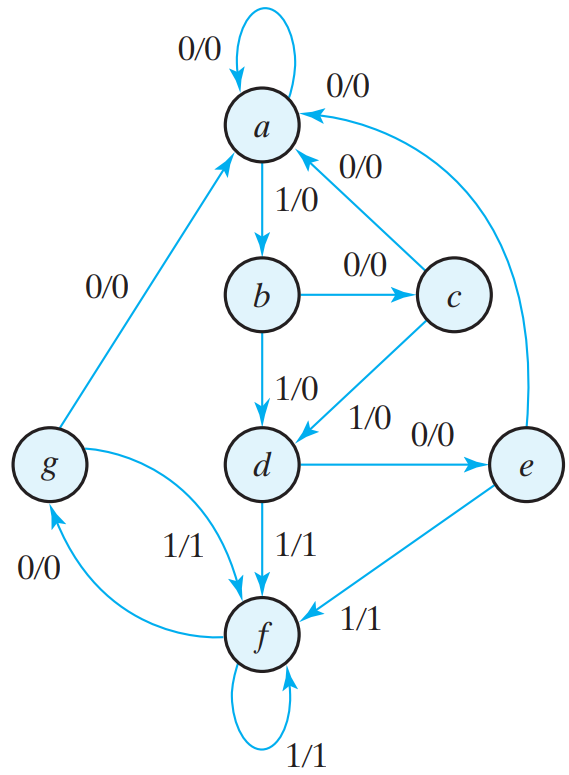
\includegraphics[width=.7\linewidth]{img/fig-5.25.png}
  \caption{A state diagram}
  \label{fig:fig5.25}
\end{figure}
The state table of the diagram is the following:
\begin{figure}[H]
  \centering
  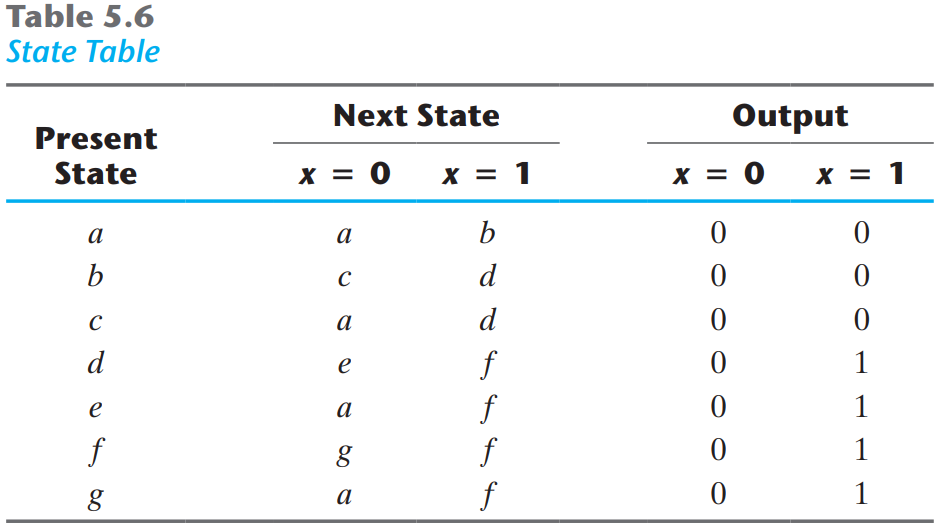
\includegraphics[width=\linewidth]{img/table-5.6.png}
  \label{table:5.6}
\end{figure}

States $e$ and $g$ are equal since for each member of the set of inputs, they give the same output and send the circuit either to the same state or an equivalent state. So one of them can be removed. So, state $g$ is removed and replaced by state $e$:
\begin{figure}[H]
  \centering
  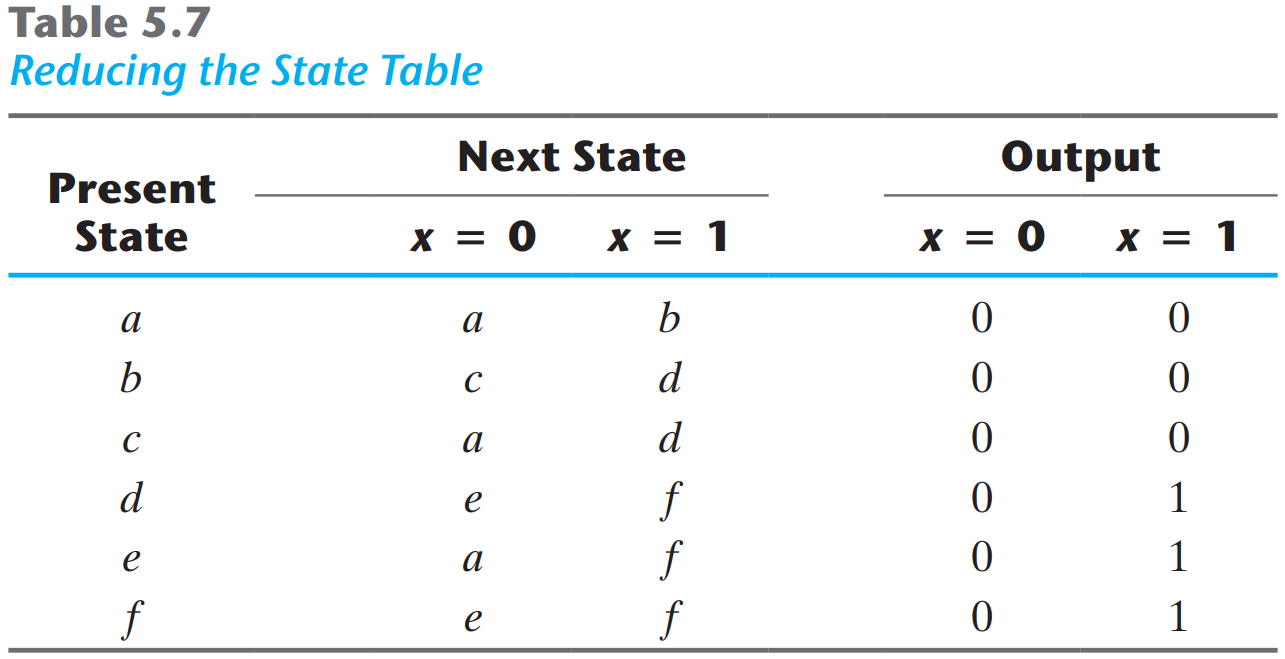
\includegraphics[width=\linewidth]{img/table-5.7.png}
  \label{table:5.7}
\end{figure}
Notice that, a state equivalence is formed. State $d$ and $f$ are equivalent. So, we can remove $f$ and replaced it with $d$:
\begin{figure}[H]
  \centering
  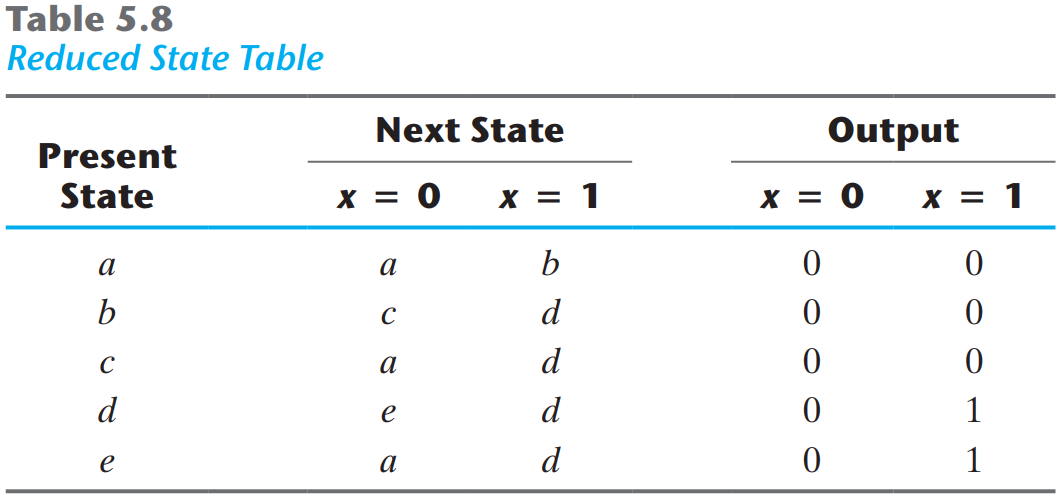
\includegraphics[width=\linewidth]{img/table-5.8.png}
  \label{table:5.8}
\end{figure}
